% !TEX program = pdflatex
% !TEX enableSynctex = true
\documentclass[aspectratio=169,10pt]{beamer}

%%%%%%%%%%%%%%%
\usepackage{booktabs}
\usepackage{xspace}
\usepackage{ulem}
\usepackage{subfig}
\usepackage{graphicx}
\usepackage{multirow}
\usepackage[capitalise,noabbrev]{cleveref} 
\usepackage{datatool}
\usepackage{algorithm} 
\usepackage{algpseudocode} 
\usepackage{empheq}
\usepackage[many]{tcolorbox}
\usepackage[capitalise,noabbrev]{cleveref}
\usetheme[progressbar=frametitle,block=fill]{metropolis}

\newcommand{\themename}{\textbf{\textsc{metropolis}}\xspace}
\definecolor{emphcolorval}{rgb}{0.23,0.4,0.7}
\definecolor{highlightcolorval}{rgb}{1,0,0}
% Penn colors
\definecolor{PennRed}{RGB}{149, 0, 26}
\definecolor{PennBlue}{RGB}{1, 37, 110}

\setbeamercolor{frametitle}{bg=PennBlue}
\setbeamercolor{progress bar}{fg=PennBlue}
\setbeamercolor{math text}{fg=PennRed}

\setbeamercolor{block title}{fg=PennBlue}
\setbeamercolor{block body}{fg=PennBlue}

\setbeamercolor{block title example}{fg=PennBlue}
\setbeamercolor{block body example}{fg=PennBlue, bg=yellow}

\setbeamersize{text margin left=5.5pt, text margin right=5.5pt}

\definecolor{cosmiclatte}{rgb}{1.0, 0.99, 0.95}
\setbeamercolor{background canvas}{bg=cosmiclatte}
%\titlegraphic{\hfill\includegraphics[height=0.8cm]{/Users/jesusfv/dropbox/Templates_Slides/penn_fulllogo.pdf}}
\newcommand{\emphcolor}[1]{\textbf{\textcolor{emphcolorval}{#1}}}
%\newcommand{\mathcolor}[1]{{\mathbf{\color{emphcolorval}{#1}}}}
\newcommand{\highlightcolor}[1]{{\textbf{\color{highlightcolorval}{#1}}}}

% \usepackage{natbib}
% \bibliographystyle{ecta}

\crefname{equation}{}{}
\newtheorem{proposition}{Proposition}
\newcommand\bigzero{\makebox(0,0){\text{\huge0}}}
\newcommand{\D}[1][]{\ensuremath{\boldsymbol{\partial}_{#1}}}
\newcommand{\R}{\ensuremath{\mathbb{R}}}
\newcommand{\diff}{\ensuremath{\mathrm{d}}}
\newcommand{\ex}{\ensuremath{\mathrm{ex}}}
\newcommand{\set}[1]{\ensuremath{\left\{{#1}\right\}}}
\newcommand{\indicator}[1]{\ensuremath{\mathds{1}\left\{{#1}\right\}}}
\newcommand{\condexpec}[3][]{\ensuremath{\mathbb{E}_{#1}\left[{#2} \; \middle| \; {#3} \right]}}
\newcommand{\prob}[2][]{\ensuremath{\mathbb{P}_{#1}\left( {#2} \right)}}
\newcommand{\cprob}[2]{\ensuremath{\mathbb{P}\left( {#1}\left| {#2} \right. \right)}}
\newcommand{\condcov}[2]{\ensuremath{\mathrm{cov}\left({#1} \; \middle| \; {#2} \right)}}
\newcommand{\expec}[2][]{\ensuremath{\mathbb{E}_{{#1}}\left[ {#2} \right]}}
\newcommand{\bigO}[1]{\ensuremath{\mathcal{O}(#1)}}
\newcommand{\Xdom}{\mathcal{X}}
\newcommand{\Yrange}{\mathcal{Y}}
\newcommand{\Xtrain}{\mathcal{X}_{\mathrm{train}}}
\newcommand{\Xextr}{\mathcal{X}_{\mathrm{extr}}}
\newcommand{\Xhull}{\mathrm{Hull}(\Xtrain)}
\newcommand{\Xtest}{\mathcal{X}_{\mathrm{test}}}
\newcommand{\Ltest}{\ell_{\mathrm{test}}}
\newcommand{\F}{\mathcal{F}}
\newcommand{\Resid}{\mathcal{R}}
\newcommand{\st}{\textrm{s.t.}\,}

\begin{document}
\title{{\vspace{0.4in}\hspace{0.2in}\textcolor{PennBlue}{Spooky Boundaries at a Distance: \\ \hspace*{5 mm}Inductive Bias, Dynamic Models, and Behavioral Macro}}}
\author{\hspace*{4 mm} Mahdi Ebrahimi Kahou\inst{1}\and
	Jes\'{u}s Fern\'{a}ndez-Villaverde\inst{2} \and Sebasti\'an G\'omez-Cardona\inst{3} \\ \hspace*{4 mm}  Jesse Perla\inst{4} \and Jan Rosa\inst{4}}

\institute{ \inst{\bf \hspace{0.2in} Conference on Frontiers in Machine Learning and Economics, Federal Reserve Bank of Philadelphia } \and
	\inst{\hspace{0.2in}1}Bowdoin College\and
	\inst{\hspace{0.2in}2}University of Pennsylvania \and
	\inst{\hspace{0.2in}3}Morningstar, Inc. \and
	\inst{\hspace{0.2in}4} University of British Columbia}


\date{}

\maketitle

\section{\textcolor{PennBlue}{Motivation, Question, and Contribution}}

\begin{frame}{Motivation}
	\begin{center}
		\emphcolor{In the long run, we are all dead---{\it J.M. Keynes, A Tract on Monetary Reform (1923)}}
		%I  will come back to this couple of time during the talk
	\end{center}
	\begin{itemize}
		\item Numerical solutions to dynamical systems are central to many quantitative fields in economics.
		% such as macroeconomics, empirical Industrial organization, urban economics, and spatial economics
		\vspace{0.1in}
		\item Dynamical systems in economics are \emphcolor{boundary value} problems:
		%unlike mnay problems natural sciences and engineering :
		\vspace{0.1in}
		\begin{enumerate}
				\item The boundary is at \emphcolor{infinity}.
				\vspace{0.05in}
				\item The values at the boundary are potentially \emphcolor{unknown}.
				\vspace{0.05in}  
		\end{enumerate}
		\item Resulting from \emphcolor{forward looking} behavior of agents.
		% and it is requirement for optimality
		\vspace{0.1in}
		\item Examples include the \emph{{\it transversality}} and the \emph{\it  no-bubble} condition.
		% No ponzi scheme
		\vspace{0.1in}
		\item Without them, the problems are \emph{ill-posed} and have infinitely many solutions: 
		\vspace{0.1in}
		\begin{itemize}
			\item The problems are ill-posed in the Hadamard sense, meaning the solutions are not unique.
			\item These forward-looking boundary conditions are a key limitation on increasing dimensionality.
		\end{itemize}
			% what do I mean by that, if it wasnt a boundary condition at infinity, I could easily solve a 1000 dimensional initial value problem 
	\end{itemize}
\end{frame}


\begin{frame}{Question}
	\emphcolor{Question}:
	\hspace{200mm}
	
	\begin{quote}
			Can we (economists and agents) \emphcolor{ignore} these long-run boundary conditions and still have accurate short/medium-run dynamics disciplined by these long-run conditions?
	\end{quote}
\end{frame}



\begin{frame}{Contribution}
	
\begin{enumerate}
	\item \emphcolor{Yes}, it is possible to meet
	long-run boundary conditions \emphcolor{without} strictly enforcing them as a constraint on the model’s dynamics.
	\vspace{0.05in}
	\begin{itemize}
		\item We show how using Machine Learning (ML) methods achieve this method.
		\vspace{0.025in}
		\item This is due to the \emphcolor{inductive bias} of ML methods.
		\vspace{0.025in} 
		\item In this paper focusing on \emph{deep neural networks}
		\vspace{0.025in} 
	\end{itemize} 
	\item We argue how inductive bias can serve as a micro-foundation for modeling forward-looking behavioral agents.
	\vspace{0.025in}
	\begin{itemize}
		\item Easy to compute. 
		\vspace{0.025in}
		\item Provides short-run accuracy.
		\vspace{0.025in}
		\item Satisfies the necessary long-run constraints.
	\end{itemize}
\end{enumerate}

\end{frame}

\section{\textcolor{PennBlue}{Background: Economic Models, Deep learning and inductive bias}}


\begin{frame}
	\frametitle{Economic Models: functional equations}
	Many theoretical models can be written as functional equations:
	\begin{itemize}
		\item Economic object of interest: $f $ where $f : \Xdom\to \mathcal{R}\subseteq \mathbb{R}^N$ 
		\begin{itemize}
			\item e.g., asset price, investment choice, best-response, etc.
		\end{itemize}
			\vspace{0.1in}
		\item Domain of $f$: $\Xdom$  
		\begin{itemize}
			\item e.g. space of dividends, capital, opponents state or time in sequential models.
		\end{itemize}
			\vspace{0.1in}
		\item The ``model'' error:  $\ell \big(x,f\big) = \mathbf{0}$,  for all $x\in \Xdom$  
		\begin{itemize}
			\item e.g., Euler and Bellman residuals, equilibrium FOCs.
		\end{itemize}
		\vspace{0.1in}
	\end{itemize}
	Then a \emphcolor{solution} is an $f^*\in \F$ where $\ell(x,f^*) = \mathbf{0}$ for all $x \in \Xdom$.\vspace{0.1in}
\end{frame}

\begin{frame}{Approximate solution: deep neural networks }
	\begin{enumerate}
		\item Sample $\mathcal{X}$: $\mathcal{D} = \{x_1,\cdots,x_N\}$
		\vspace{0.025in}
		\item Pick a deep neural network $f_\theta(\cdot) \in \mathcal{H}(\theta)$:
		\begin{itemize}
			\item $\theta$: parameters for optimization (i.e., weights and biases).  
		\end{itemize}
		\vspace{0.025in}
		\item To find an approximation for $f$ solve:
		\begin{align*}
			\min_{\theta } \frac{1}{N}\sum_{x \in \mathcal{D}} \|\ell(x,f_\theta)\|_2^2
		\end{align*}
		\begin{itemize}
			\item Deep neural networks are highly over-parameterized.
			\item Formally, $|\theta|\gg N$ 
		\end{itemize}
	\end{enumerate}
\end{frame}

\begin{frame}{Over-parameterized interpolation}
	\begin{itemize}
		\item Over-parameterized ($|\theta|\gg N$), the optimization problem can have many solutions.
		\item Since individual $\theta$ are irrelevant it is helpful to think of optimization directly within $\mathcal{H}$
		\vspace{-0.025in}
		\begin{empheq}[box=\tcbhighmath]{equation*}
			\min_{f_{\theta} \in \mathcal{H}} \sum_{x \in \mathcal{D}} \|\ell(x,f_{\theta})\|_2^2\label{eq:functional-optimization}
		\end{empheq}
		\vspace{-0.025in}
	\item But which $f_{\theta}$?
	\item \emphcolor{Mental model:} chooses min-norm interpolating solution for a (usually) unknown functional norm $\psi$
			\vspace{-0.025in}
	\begin{empheq}[box=\tcbhighmath]{align*}
		\min_{\hat{f}\in \mathcal{H}} &||f_\theta||_\psi\\
		\st & \ell(x,f_\theta)=0,\quad \text{ for all } x \in \mathcal{D}
	\end{empheq}
	\vspace{-0.025in}
	\item That is what we mean by \emphcolor{inductive bias} (see Belkin, 2021 and Ma and Yang, 2021).
	
	\item  Characterizing $S$ (e.g., sobolev norms or semi-norms?) is an active research area in ML.
	\end{itemize}
\end{frame}

\begin{frame}{Smooth interpolation}
	\begin{itemize}
		\item Intuition: biased toward solutions which are flattest and have smallest derivatives
	\end{itemize}
		\begin{figure}[t!]
		\centering
		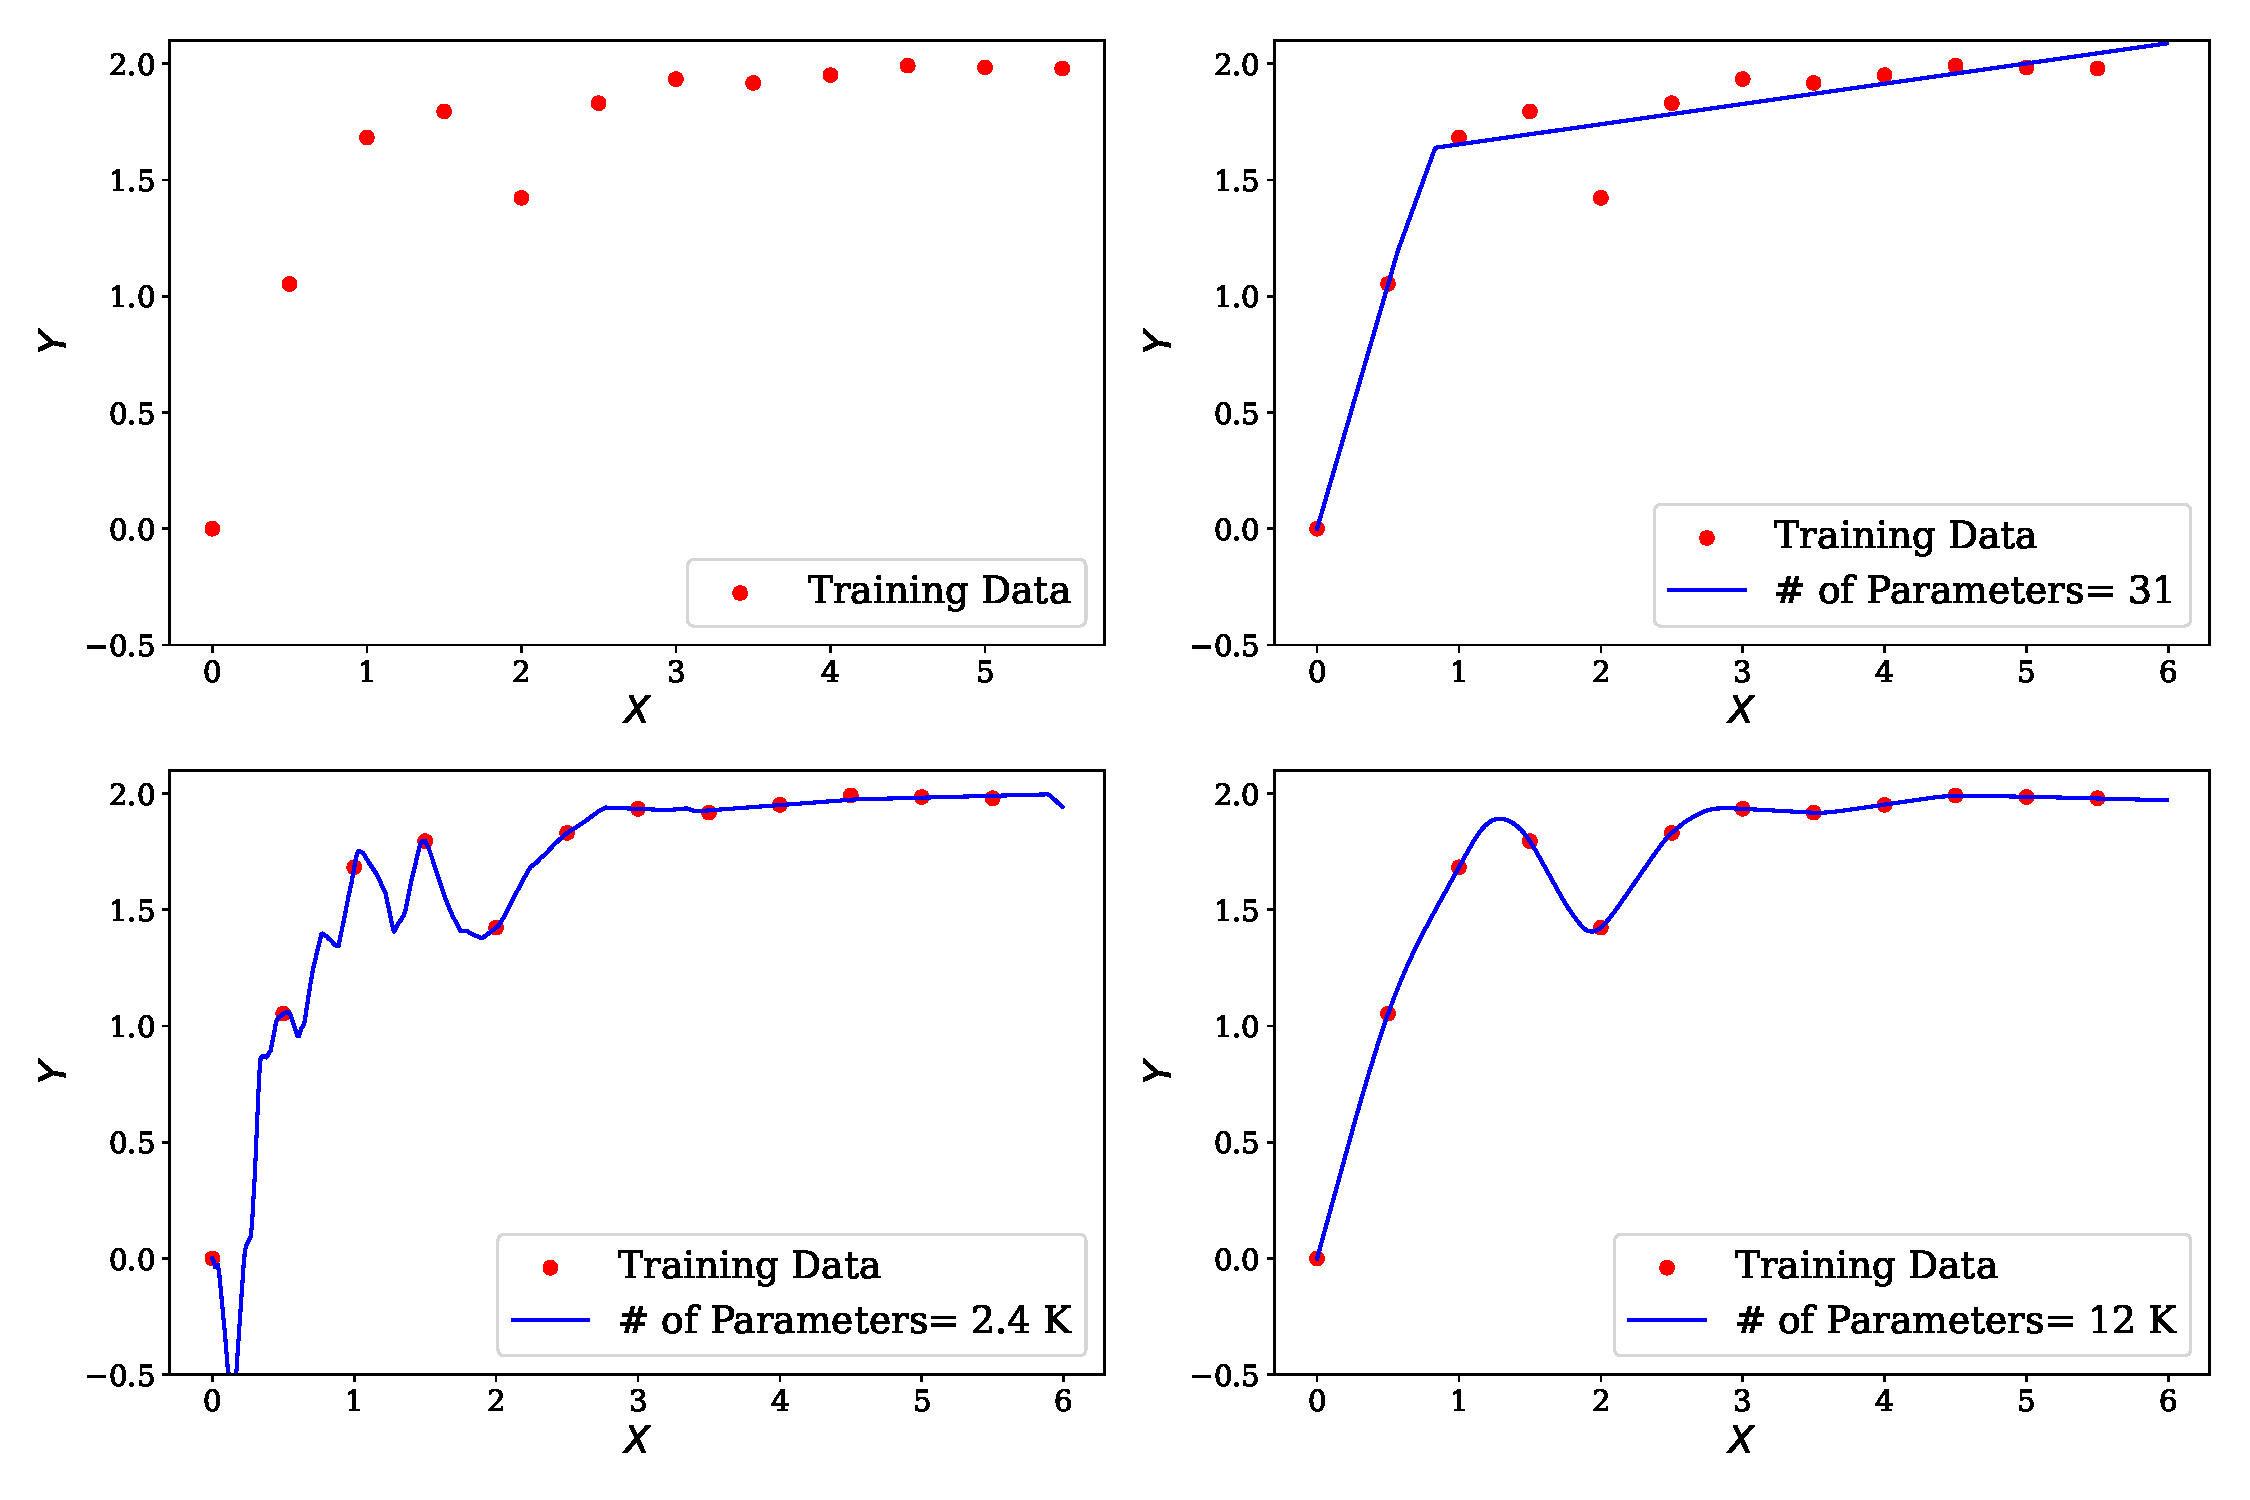
\includegraphics[width=0.65\textwidth]{figs/smooth_interpolation.pdf}
	\end{figure}
\end{frame}

\begin{frame}{Intuition of the paper}
	\begin{columns}
		\begin{column}{0.5\textwidth}
			% Content for the left column
			\begin{itemize}
				\item \emphcolor{Minimum-norm implicit bias}: 
				\begin{itemize}
					\item Over-parameterized models (e.g., large neural networks) interpolate the train data.
					%therefore they are many possible solutions
					\vspace{0.05in}
					\item They are biased towards interpolating functions with smaller norms. 
					\item So they dont like explosive functions.
				\end{itemize}
				\vspace{0.1in}
				\item \emphcolor{Violation of economic boundary conditions}:
				\begin{itemize}
					\item Sub-optimal solutions diverge (explode) over time.
					% As you can see in the plot optimal solution goe to the steady-state, the black dot, and any othe trajectory globaly or locally diveges. That is the signature of economic models
					\vspace{0.05in}
					\item They have large or explosive norms.
					% Given that they are divergent, then they are large functions with large norms
					\vspace{0.05in}
					\item This is due to the \emphcolor{saddle-path} nature of econ problems.
					% many economic models have this saddle path nature
				\end{itemize}
			\end{itemize}
		\end{column}
		\begin{column}{0.5\textwidth}
		\begin{figure}[t!]
			\centering
			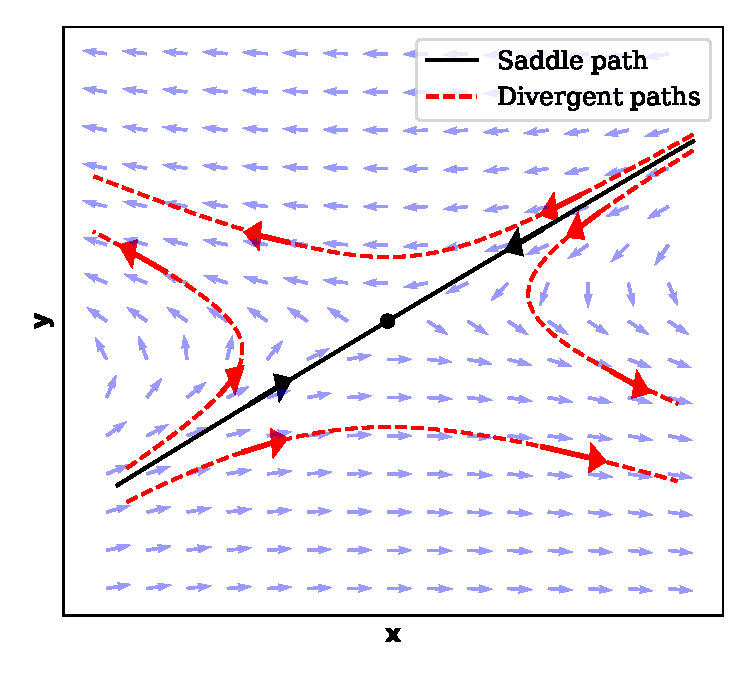
\includegraphics[width=\textwidth]{figs/saddle_path.pdf}
			\vspace{-7mm}
		\end{figure}
		\end{column}
	\end{columns}
\end{frame}

\section{Outline}

\begin{frame}{Outline of the Talk}
	
	To explore how we can ignore events after ``we are all dead'', we show deep learning solutions to
	\begin{enumerate}
		\item Classic linear-asset pricing model.\vspace{0.1in}
		\item Sequential formulation of the neoclassical growth model.\vspace{0.1in}
		\item Sequential formulation of the neoclassical growth model with non-concave production function.\vspace{0.1in}
		\item Equivalent for a recursive formulation of the neoclassical growth model.\vspace{0.1in}
		
	\end{enumerate}
\end{frame}

\section{\textcolor{PennBlue}{Linear asset pricing and he no-bubble condition}}

\begin{frame}{Linear asset pricing: setup }
	\begin{itemize}
	\item The risk-neutral price, $p(t)$, of a claim to a stream of dividends, $y(t)$, is given by
	the recursive equation:
	\begin{align*}
		p(t) = y(t) + \beta p(t+1), \quad \text{for}~ t=0,1,\cdots
	\end{align*}
	\item $\beta<1$, and $y(t)$ is exogenous.
	\item  This is a one dimensional dynamical system with unknown initial condition  $p(0)$. This problem is \emphcolor{ill-posed}.
	\item A family solutions
	 \begin{align*}
	 	p(t) = \underbrace{p_f(t)}_{\text{fundamentals}} +  \underbrace{\zeta (\frac{1}{\beta})^t}_{\text{explosive bubble}}
	 \end{align*}
	 \item $p_f(t) \equiv \sum_{\tau =0}^\infty \beta^\tau u(t+\tau)$. Each solution corresponds to a different $\zeta>0$.
	\end{itemize}
\end{frame}

\begin{frame}{Linear asset pricing: the long-run boundary condition}
	We need a condition that rule out the explosive bubbles and chooses $\zeta =0$
	\begin{align*}
		\lim_{t\rightarrow \infty} \beta^t p(t) = 0
	\end{align*}
\end{frame}

\begin{frame}{Ridgeless kernel regression}
\end{frame}
\begin{frame}{Ridgeless kernel regression: minimum Sobolev seminorm solutions}
We also solve the ridgeless kernel regression 
\begin{align*}
	\lim_{\lambda\rightarrow 0} \min_{\hat{\mathbf{x}}, \hat{\mathbf{y}}} \sum_{t_i \in \mathcal{D}} &\left[\eta_1 \left\Vert \hat{\dot{\mathbf{x}}}(t_i) 
	- \mathbf{F}(\hat{\mathbf{x}}(t_i), \hat{\mathbf{y}}(t_i)(t_i)) \right\Vert_2^2 + \eta_2 \left\Vert \hat{\dot{\mathbf{y}}}(t_i) -  \mathbf{G}(\hat{\mathbf{x}}(t_i), \hat{\mathbf{y}}(t_i)) \right\Vert_2^2\right.\nonumber\\
	&\left.+ \eta_3 \left\Vert \mathbf{H}(\hat{\mathbf{x}}(t_i), \hat{\mathbf{y}}(t_i)) \right\Vert_2^2 \right] + \eta_4 \left\Vert \hat{\mathbf{x}}(0) - \hat{\mathbf{x}}_0 \right\Vert_2^2 + \lambda \underbrace{\left[\sum_{m=1}^{N_x}\Vert \hat{\dot{\mathbf{x}}}^{(m)}\Vert^2_{\mathcal{H}}+ \sum_{m=1}^{N_y}\Vert \hat{\dot{\mathbf{y}}}^{(m)}\Vert^2_{\mathcal{H}}\right]}_{\text{The Sobolev semi-norm}}
\end{align*}
\begin{itemize}
	\item Targeting Sobolev semi-norm.
	% minimizing the norm of the derivative
	\vspace{0.1in}
	\item This choice is very natural: it solves the instability issues of the classical algorithm.
	%because of the saddle path-nature of the problems divergent and explosive functions have large derivatives therefore we kick out those
\end{itemize} 
\end{frame}

\section{Applications}

\begin{frame}{Linear asset pricing}
	%why this probelm? Not because this problem is hard. But that is the first model that is the simplest model that incorporates bubbles in economics
\begin{align}
	\dot{\mathbf{x}}(t) &= c + g \mathbf{x}(t) \label{eq:asset-pricing-x-dot}\\%:= \mathbf{F}(\mathbf{x}(t), \mathbf{y}(t))
	\dot{\mathbf{y}}(t) &= r \mathbf{y}(t) - \mathbf{x}(t)  \label{eq:asset-pricing-y-dot}\\%:= \mathbf{G}(\mathbf{x}(t), \mathbf{y}(t))
	0 &= \lim_{t\rightarrow \infty} e^{-r t}\mathbf{y}(t) \label{eq:asset-pricing-no-bubble}%:= \mathbf{B}(\mathbf{x}(t), \mathbf{y}(t))
\end{align}

\begin{itemize}
	\item $\mathbf{x}(t)\in \mathbb{R}$: dividends, $\mathbf{y}(t)\in \mathbb{R}$: prices, and $\mathbf{x}_0$ given. 
	\vspace{0.1in}
	\item Equation \cref{eq:asset-pricing-x-dot}: how the dividends evolve in time.
	\vspace{0.1in}
	\item  Equation \cref{eq:asset-pricing-y-dot}: how the prices evolve in time.
	\vspace{0.1in}
	\item Equation \cref{eq:asset-pricing-no-bubble}: ``no-bubble" condition, the boundary condition at infinity. 
	\end{itemize}
\end{frame}

\begin{frame}{Why do we need the boundary condition?}
	%Imagine if I didnt have the boundary condition, what would happen?
	\begin{align*}
		\dot{\mathbf{x}}(t) &= c + g \mathbf{x}(t) \\
		\dot{\mathbf{y}}(t) &= r \mathbf{y}(t) - \mathbf{x}(t)
	\end{align*}
	\begin{itemize}
		\item The solutions: 
		\begin{align*}
			\mathbf{y}(t) = \mathbf{y}_f(t) + \zeta e^{rt}
		\end{align*}
		\item $\mathbf{y}_f(t) = \int_0^\infty e^{-r\tau} \mathbf{x}(t+s)ds$: price based on the fundamentals.
		\vspace{0.1in}
		\item $\zeta e^{rt}$: explosive bubble terms, it has to be \emphcolor{ruled out} by the boundary condition.
		%doesnt correspond to any economic variable
		\vspace{0.1in} 
		\item Triangle inequality: $\Vert \mathbf{y}_f\Vert < \Vert \mathbf{y}\Vert$.
		%go with any norm, because of the positivity and addtive structure 
		\vspace{0.1in}
		\item The price based on the fundamentals has the \emphcolor{lowest norm}.
	\end{itemize}
\end{frame}









\begin{frame}{Conclusion}
	\begin{itemize}
		\item Long-run (\emphcolor{global}) conditions can be replaced with appropriate regularization (\emphcolor{local}) to achieve the optimal solutions.
		\vspace{0.1in}
		\item The minimum-norm implicit bias of large ML models aligns with optimality in economic dynamic models.
		\vspace{0.1in}
		\item Both kernel and neural network approximations accurately learn the right steady state(s).
		\vspace{0.1in}
		\item Proceeding with \emphcolor{caution}: can regularization be thought of as an equilibrium selection device?
		%if we are about to translate economic dynamic models into an ERM, can regularization act as an equilibrium device? Think about it, ERM in statistical learning or machine learning is about two things: uniform of law of large numbers and capacity control (so what are going to do about this capacity control regularization)
	\end{itemize}
\end{frame}

\section{Appendix}


\end{document}
